\documentclass[conference]{IEEEtran}
\IEEEoverridecommandlockouts
\usepackage{cite}
\usepackage{amsmath,amssymb,amsfonts}
\usepackage{algorithmic}
\usepackage{graphicx}
\usepackage{textcomp}
\usepackage{booktabs} 
\usepackage{xcolor}
\usepackage{geometry}
\usepackage{hyperref}
\geometry{margin=0.1in}
\def\BibTeX{{\rm B\kern-.05em{\sc i\kern-.025em b}\kern-.08em
    T\kern-.1667em\lower.7ex\hbox{E}\kern-.125emX}}
\begin{document}

\title{\Large{\textbf{LEPL1110 :}} \Large{\textbf{\textit{Analyse et simulation numérique d'un problème d'élasticité linéaire}}}\\
\normalsize{\textit{Assistant:} \textbf{YANS} Simon - \textit{Tuteur:} \textbf{DONY} Gatien - \textit{Professeur:} \textbf{LEGAT} Vincent} \\
\normalsize{\textit{Etudiant n°1:} \textbf{DELSART} Mathis (\textbf{31302100}) - \textit{Etudiant n°2:} \textbf{ANTONUTTI} Adrien (\textbf{31202100}) - \textit{Numéro de groupe:} \textbf{75}}}

\maketitle 

\vspace*{-2cm}

\section{Comparaison des solveurs et des renumérotations}

Le solveur plein présente des performances insuffisantes pour traiter un maillage comportant un grand nombre d'éléments. Pour remédier à cela, nous avons adopté le solveur bande, qui exploite la symétrie de la matrice en ne considérant que sa partie supérieure. Plus la bande de la matrice est étroite, plus la résolution du système linéaire est rapide. Pour atteindre cet objectif, plusieurs techniques de renumérotation sont envisageables. Les approches les plus simples consistent à renuméroter les nœuds selon leur composante X ou Y. Bien que fonctionnelles, ces méthodes ne sont pas optimales pour toutes les géométries. L'algorithme de renumérotation RCMK (reverse Cuthill–McKee) permet d'obtenir une renumérotation optimale pour toutes les configurations géométriques, conduisant à la plus petite bande possible. L'élimination de Gauss d'un solveur plein a une complexité de O($n^3$), tandis que celle d'un solveur bande est en O($n^2$) si la largeur de bande est bien inférieure à $n$, le nombre de noeuds. De plus, avec une renumérotation efficace, la largeur de la bande de la matrice évolue en O($\sqrt{n}$), sinon en O($n$).

La figure \ref{fig:BandFullRenum} illustre les temps d'exécution du programme avec les solveurs plein et bande et les compare à la complexité attendue, en utilisant trois méthodes de renumérotation différentes (X, Y et RCMK). Elle présente également l'évolution de la taille de la bande pour chaque méthode de renumérotation. Ces résultats ont été obtenus en utilisant la géométrie de notre pont avec un maillage de taille constante.

\begin{figure}[!htb]
    \centering
    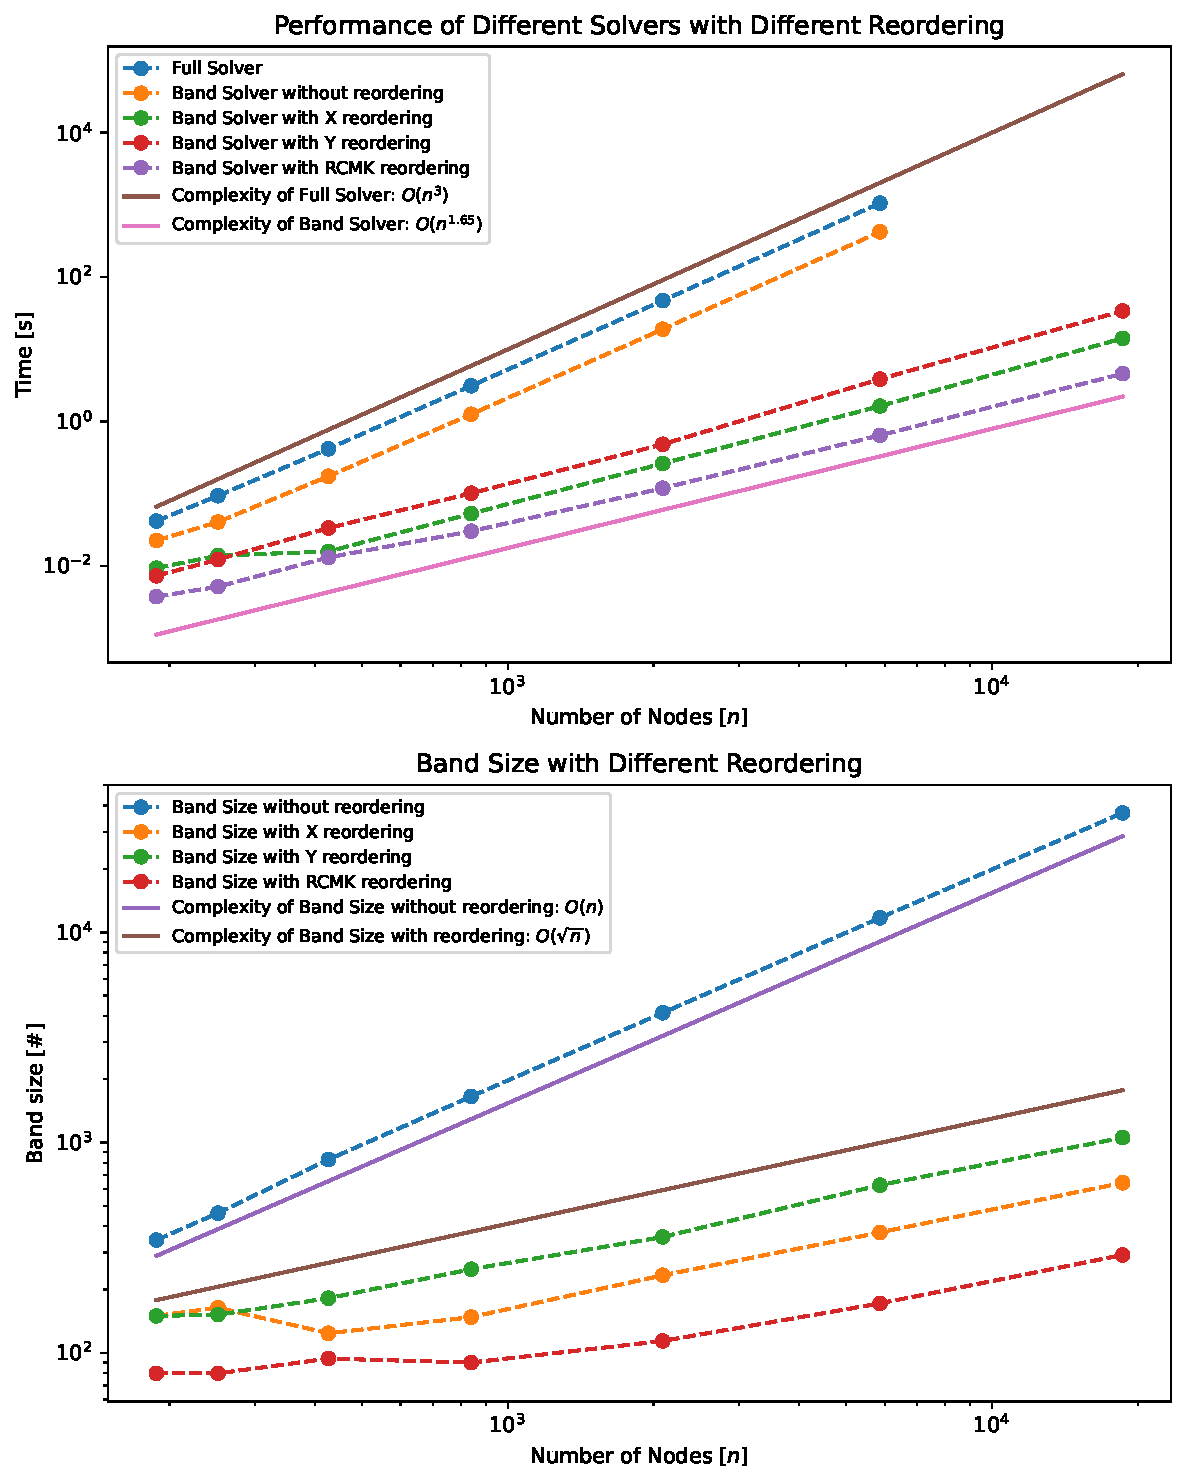
\includegraphics[width=8.5cm]{Figures/solver_plot.pdf}
    \label{fig:BandFullRenum}
\end{figure}

\section{Validation du code}

Afin de valider notre code, nous avons choisi une géométrie de poutre encastrée sur son côté gauche (ce qui implique des déplacements nuls selon les axes X et Y). Sur le dessus de la poutre, une densité de force dirigée vers le bas de 1250 kN/m a été appliquée uniformément. La poutre, en acier, mesure 8 m de longueur, 1 m de hauteur et possède une section carrée. L'objectif est de déterminer la déformation de la poutre, qui décrit sa forme sous l'effet des charges appliquées.

La solution analytique de ce problème est dérivée de la théorie des poutres. Elle est donnée par l'équation : $y(x) = \frac{- w x^2}{24 E I} (x^2 - 4 L x + 6 L^2)$
où E représente le module de Young (211 GPa pour l'acier), w est la densité de force appliquée le long de la poutre, L est sa longueur, et I est le moment quadratique de la section transversale, égal à $\frac{h^4}{12}$. \\

La figure \ref{fig:validationCode_Beam} illustre le résultat obtenu par notre simulation. Le facteur de déformation a été ajusté à 100 pour la simulation ainsi que pour la solution analytique. Nous constatons une concordance remarquable entre la courbure analytique prédite et la solution numérique, ce qui confirme la validité de notre code pour les conditions aux limites spécifiées et pour le cas de tension plane. Nous avons également vérifié cette validité en appliquant une condition de Dirichlet NT sur le côté gauche et une condition de Neumann Y sur le dessus, obtenant les mêmes résultats, ce qui valide les conditions normales et tangentielles.

\begin{figure}[!htb]
    \centering
    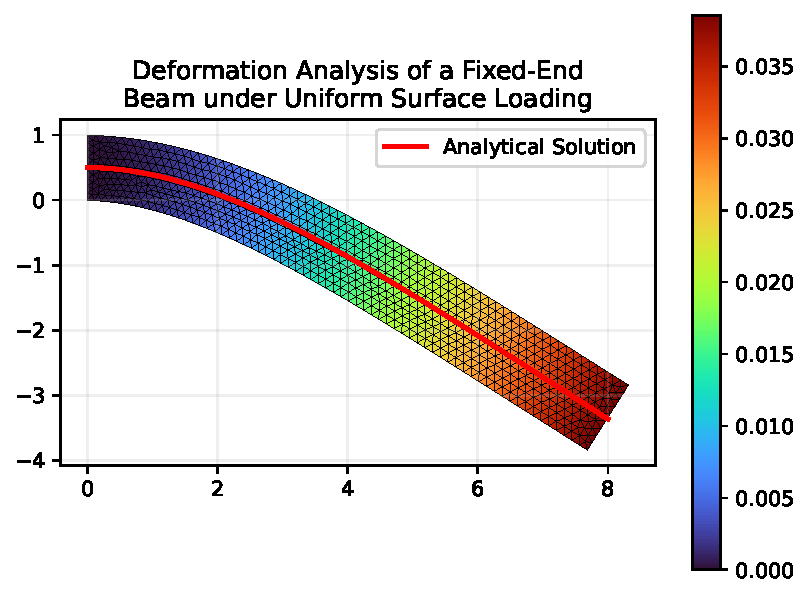
\includegraphics[width=8.5cm]{Figures/poutre_validation_code.pdf}
    \label{fig:validationCode_Beam}
\end{figure}

\section{Analyse de convergence}


Pour analyser la convergence, nous avons utilisé la géométrie de la poutre étudiée précédemment. Nous avons comparé l'erreur numérique de la simulation à une solution de référence obtenue avec le maillage le plus raffiné possible. Pour chaque maillage de taille constante, nous avons calculé la norme de la déformation moyenne par noeud, représentée par $u_{mean} = \frac{1}{n} \sqrt{\sum\limits_{i=1}^{n} u_{x,i}^{2} + \sum\limits_{i=1}^{n} u_{y,i}^2}$ où n est le nombre de noeud du maillage et $u_{x,i}$ et $u_{y,i}$ sont respectivement les déformations en X et en Y du noeud i. En calculant l'erreur $\epsilon = (u_{mean} - u_{ref})^2$, nous avons pu évaluer la convergence. Les résultats, présentés à la figure \ref{fig:convergence} montrent une diminution de l'erreur avec la réduction de la taille du maillage, conformément à nos attentes, mais avec une vitesse variable.
En analysant les pentes des courbes en échelle logarithmique, nous avons déduit l'ordre de convergence. En effet, on a $\epsilon(h) = h^p$ où p est l'ordre de convergence. En échelle logarithmique, cette équation devient $log(\epsilon(h)) = p * log(h) + C_{ste}$.

Nous pouvons observer que l'ordre de convergence est d'environ 0.75 pour les maillages grossiers, suggérant une convergence plus lente. En revanche, pour des maillages plus fins, l'ordre de convergence est d'environ 2, indiquant une convergence plus rapide à mesure que la taille du maillage diminue.

\begin{figure}[!htb]
    \centering
    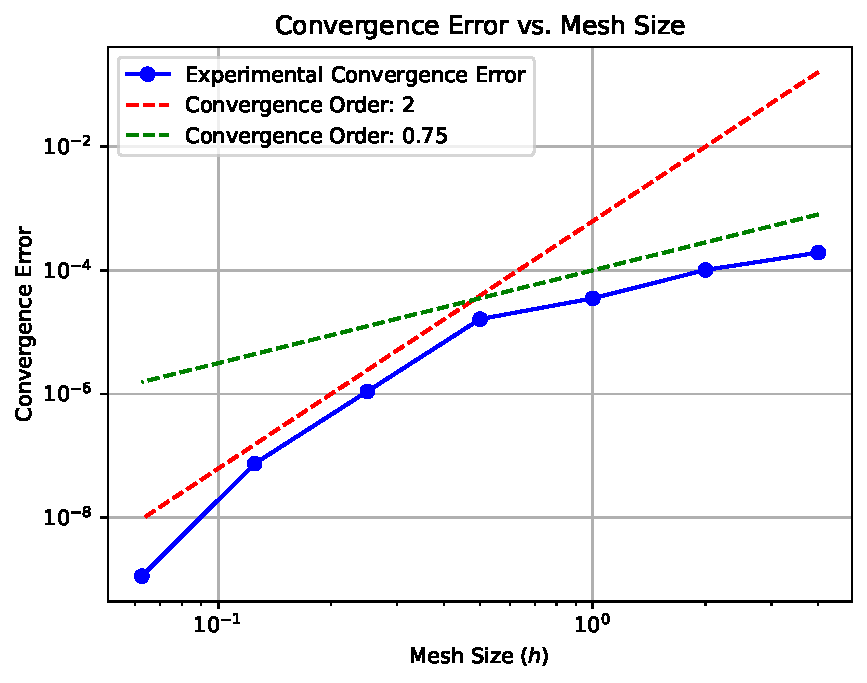
\includegraphics[width=8.5cm]{Figures/convergence_plot.pdf}
    \label{fig:convergence}
\end{figure}

\section{Analyse de la physique d'un pont}

Notre pont associe les caractéristiques des ponts à haubans et des ponts en arcs, ce qui confère à sa structure une complexité et une robustesse uniques. Dans un pont à haubans, plusieurs pylônes soutiennent des câbles qui redirigent les forces vers les pylônes pour supporter le poids du tablier et de sa charge, entraînant des contraintes importantes dans les câbles. En revanche, un pont en arc est constitué d'une ou plusieurs voûtes, répartissant la charge du tablier en compression sur les piliers du pont.

\section{Résultats et interprétations}

Pour les deux sous-sections suivantes, nous avons simulé un embouteillage en plaçant quatre camions à l'arrêt sur le pont, avec deux camions occupant la même zone pour tenir compte des deux voies en profondeur du pont. Sur le passage piétonnier, nous avons simulé le passage de piétons en considérant un piéton pesant 70 kg par mètre carré. Cela nous donne une densité de charge constante de 38 kN/m sur le pont et de 4800 N/m sur le passage piétonnier (le pont ayant une largeur de 7 mètres). Le facteur de déformation pour les graphiques est de 20000.

\subsection{Déformation maximale}

Nous pouvons observer sur la figure \ref{fig:elasticityBridge} la déformation du pont sous une charge uniforme. La déformation maximale, de l'ordre de 0,01 mm, se situe au niveau du passage piétonnier qui est l'endroit le moins soutenu. Les déformations minimes du tablier principal s'expliquent par le soutien significatif apporté par les câbles. En effet, les câbles compensent efficacement la déformation en exerçant une force de tension. Nous approfondirons cette analyse dans la section suivante.

\begin{figure}[!htb]
    \centering
    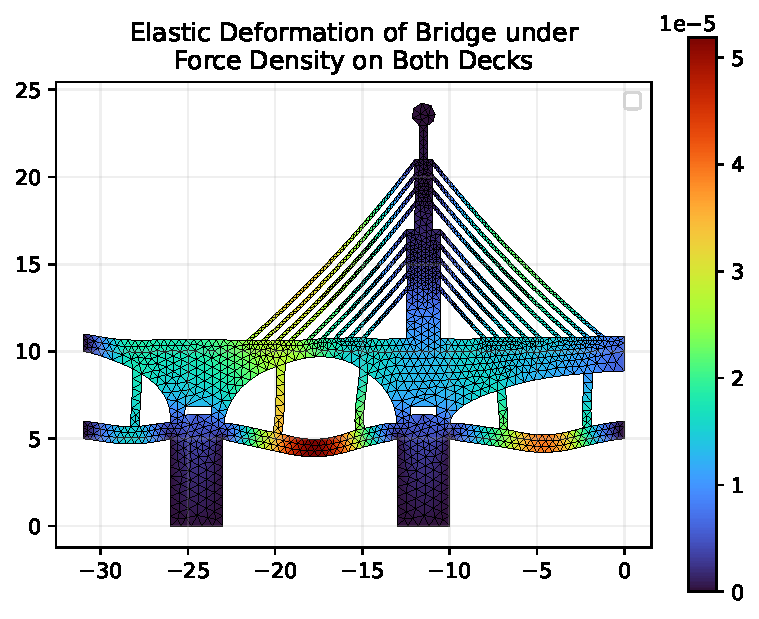
\includegraphics[width=8.5cm]{Figures/elasticityBridge.pdf}
    \label{fig:elasticityBridge}
\end{figure}

\subsection{Critère de plasticité}

Nous avons calculé les tensions $\sigma_{xx}$, $\sigma_{yy}$ et $\sigma_{xy}$ en chaque nœud de notre structure. Pour interpréter ce champ vectoriel, nous avons utilisé le critère de Von Mises, qui permet de passer d'une grandeur vectorielle à une grandeur scalaire. Ce critère est calculé en faisant la somme des éléments au carré de la matrice $\sigma - \mathrm{Tr} (\sigma)  I$ multipliée par un facteur de $\frac{3}{2}$ et mise sous la racine carrée. Lorsque la valeur du critère de Von Mises dépasse la limite d'élasticité du matériau, celui-ci subit une déformation plastique et donc irréversible. Pour l'acier, cette limite est généralement fixée autour de 250 MPa.

En examinant la figure \ref{fig:maxConstrainsBridge}, nous observons que les contraintes les plus significatives se trouvent au niveau des câbles. Celles-ci s'expliquent par le fait qu'ils travaillent principalement en tension. En revanche, les tabliers du pont supportent les charges en compression, ce qui peut entraîner des déformations plus importantes plutôt que des contraintes très élevées. La contrainte maximale observée est de 50MPa, soit 5 fois moins élevée que la limité d'élasticité du pont.

\begin{figure}[!htb]
    \centering
    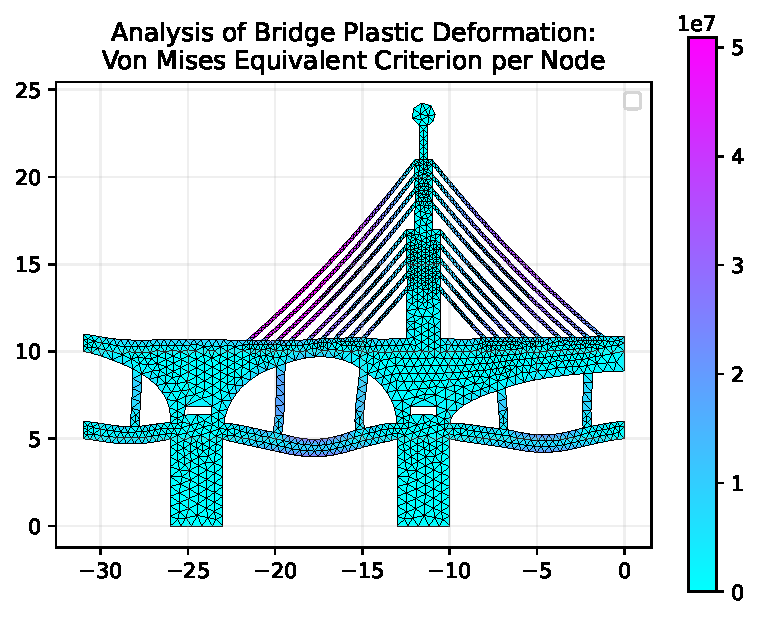
\includegraphics[width=9cm]{Figures/maxConstrainBridge.pdf}
    \label{fig:maxConstrainsBridge}
\end{figure}

\section{Animations}

Dans les deux premières simulations, nous avons appliqué une charge uniforme très élevée sur les tabliers de deux ponts différents. Dans la première simulation, le pont est équipé de câbles de soutien, tandis que dans la deuxième simulation, ces câbles sont absents. Nous avons observé que la déformation maximale du pont est beaucoup plus faible dans le cas où les câbles sont présents, ce qui démontre leurs capacités à absorber une partie importante de la déformation sous contrainte. Cependant, dans le cas du pont sans câble, la déformation est beaucoup plus prononcée, avec un point sensible situé du côté droit où l'arc est plus allongé et plus bas. En revanche, sur le pont avec les câbles, le point sensible se trouve à gauche, car c'est l'endroit le moins soutenu par les câbles. Il est important de noter que le facteur de déformation est significativement plus élevé dans la première simulation (10000 par rapport à 4000), ce qui indique une plus grande résistance du pont avec les câbles par rapport à celui sans câble.

Dans la troisième simulation, nous avons simulé le déplacement d'une charge le long de l'axe des x, simulant ainsi le passage d'une voiture à vitesse constante. Pour réaliser cette simulation, nous avons ajouté une fonction qui ajustait la densité de force appliquée sur le tablier en fonction de la position X du noeud et de l'image actuelle de l'animation. Nous avons pu observer le point sensible à gauche du pont, et nous avons remarqué que les câbles jouaient un rôle crucial en supportant une partie importante de la charge, réduisant ainsi la déformation globale du pont.

Vous pouvez visionner ces trois simulations sur YouTube en suivant ce lien : \href{https://youtu.be/QxjO2Oo-mYU}{https://youtu.be/QxjO2Oo-mYU}.

\end{document}